\section{Theorie}
\label{sec:Theorie}

\subsection{Wechselwirkung von Photonen mit Materie}

Tritt ein Photon $\gamma$ in Materie ein, so kann es mit Atomkernen oder Elektronen wechselwirken. Ein Maß für die Wahrscheinlichkeit von 
einer solchen Wechselwirkung ist der Wirkungsquerschnitt $\sigma$, welcher proportional zum Extinktionskoeffizienten $\mu = \frac{1}{\bar{x}} \propto \sigma$
ist. Dabei ist $\bar{x}$ die mittlere freie Weglänge. Für die Strahlintensität gilt mit $\mu$

\begin{equation}
    N\left(D\right) = N_0 \exp{-\mu D}
    \label{eqn:Strahl}
\end{equation}

nach Durchdringen einer Absorberschicht der Dicke $D$ mit ursprünglicher Strahlintensität $N_0$.\\

Es gibt drei besonders relevante Wechselwirkungsprozesse für die $\gamma$-Spektroskopie. Der Photo- und Comptoneffekt und die Paarbildung.

\subsubsection{Photo-Effekt}

Beim Photo-Effekt wechselwirkt ein $\gamma$-Quant mit einem Hüllenelektron. Aus Impulserhaltungsgründen tut es dies bevorzugt mit Elektronen der 
K-Schale. Damit dies geschehen kann, muss die Energie des Photons $E_\gamma$ mindestens so groß wie die Bindungsenergie des Elektrons $E_B$ sein, 
um dieses aus seinem Zustand zu entfernen. Falls $E_\gamma > E_B$ gilt, erhält das Elektron als kinetische Energie $E_\gamma - E_B$. Das "Loch", 
das durch diesen Prozess entsteht, wird durch ein Elektron aus einer höheren Schale ausgefüllt und das so entstehende Loch wiederem durch ein 
Elektron einer noch höheren Schale etc. Dabei werden charakteristische Röntgen-Strahlung emittiert, die den Absorber jedoch nur in seltenen 
Fällen verlässt, sodass das gesamte $E_\gamma$ in diesem verbleibt. Der Wirkungsquerschnitt ist dabei gegeben mit 

\begin{equation*}
    \sigma_{Ph} = Z^\alpha E^\delta,
\end{equation*}

wobei $\num{4}<\alpha<\num{5}$ und $\delta \approx \num{3.5} $.

\subsubsection{Compton-Effekt}

Der Compton-Effekt beschreibt die unelastische Streuung eines Photons an einem ruhenden Elektron. Dabei gibt das Photon ein Teil seiner Energie ab 
und ändert seine Ausbreitungsrichtung. Mithilfe des Energie- und Impulserhaltungssatzes lässt sich die Energie des gestoßenen Elektrons zu 

\begin{equation*}
    E_l = E_\gamma \frac{\epsilon\left(1-\cos{\theta}\right)}{1+\epsilon\left(1-\cos{\theta}\right)}
\end{equation*}

mit $\epsilon = \frac{E_\gamma}{m_0 c^2}$ und $\theta \angle (\vec{p_\gamma}, \vec{p_{e'}})$ bestimmen. Bei $\theta = 180°$ beträgt der 
maximale Energieübertrag somit

\begin{equation*}
    E_{l,max} = E_\gamma \frac{2\epsilon}{1+2\epsilon}.
    \label{eqn:Kante}
\end{equation*}

Demnach gilt für alle $\theta$ $E_l < E_\gamma$. Der Wirkungsquerschnitt ergibt sich zu 

\begin{equation*}
    \sigma_{Co} = \frac{3}{4}\sigma_{Th}\left(1-2\epsilon+\frac{26}{5}\epsilon^2+\ddots\right)
\end{equation*}

mit 

\begin{equation*}
    \sigma_{Th} = \frac{8}{3}\pi r_e^2.
\end{equation*}

Dabei ist $r_e$ der klassische Elektronenradius. Für $\epsilon\rightarrow 0$ gilt $\sigma_{Co} \approx \sigma_{Th}$.

\subsubsection{Paarbildung}

Die Paarbildung kann stattfinden, wenn $E_\gamma>2m_0c^2$ gilt, wenn ein Atom der Stoßpartner ist oder wenn $E_\gamma > 4m_0c^2$, falls 
ein Elektron der Stoßpartner ist. Dabei wandelt sich das Photon unter Anwesenheit des Stoßpartners in ein Elektron und Positron um, 
auf die sich aufgrung der Impulserhaltung die übrige Energie gleichmäßig in Form kinetischer Energie verteilt. Der Wirkungsquerschnitt
der Paarbildung lässt sich durch 

\begin{align*}
    \sigma_{\symup{Pa}} &= \alpha r_e^2 z^2\left(\frac{28}{9}\ln{\left(2\epsilon\right)}-\frac{218}{27}\right)\textrm{Verschwindene Abschirmung}\\
    \sigma_{\symup{Pa}} &= \alpha r_e^2 z^2\left(\frac{28}{9}\ln{\left(\frac{183}{z^{3/2}}\right)}-\frac{2}{27}\right) \textrm{Vollständige Abschirmung}
\end{align*}

für die beiden Extremfälle verschwindender (bei $10<E_\gamma<\SI{25}{\mega\eV}$) oder vollständiger Abschirmung (bei $\SI{500}{\mega\eV}<E_\gamma$) beschreiben.

\subsubsection{Extinktionskoeffizient}

Aus den Wirkungsquerschnitten lassen sich die Extinktionskoeffizienten bestimmen. Abbildung \ref{fig:Ext} zeigt die Energieabhängigkeit des Extinktionskoeffizient
für Germanium getrennt nach den verschiedenen Wechselwirkungsprozessen.

\begin{figure}
    \centering
    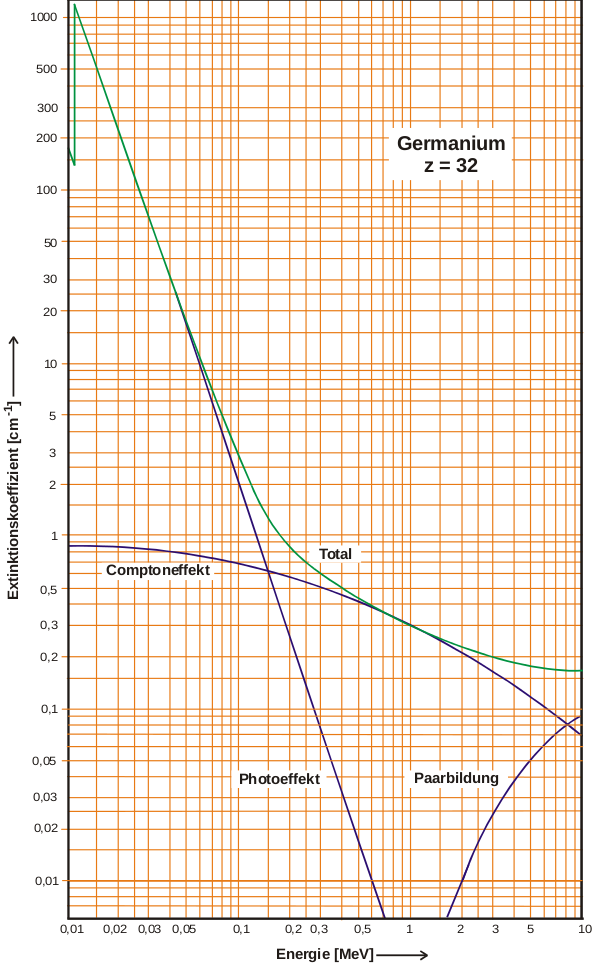
\includegraphics[scale=0.3]{content/Ext.png}
    \caption{Energieabhängigkeit des Extinktionskoeffizient für Germanium getrennt nach den verschiedenen Wechselwirkungsprozessen [1].}
    \label{fig:Ext}
\end{figure}

\subsection{Aufbau und Wirkungsweise eines Germanium Detektors}

Der Germanium Detektor ist ein Halbleiterdetektor. Demnach besteht dieser im Wesentlichen aus einer Halbleiterdiode. Im Detekorkristall 
existieren zwei aneinandergrenzende Bereiche die p- und n-dotiert sind. Durch Rekombination der Ladungsträger entsteht eine ladungsträgerarme 
Zone. Die übrig gebliebenen Akzeptoren bzw. Donatoren bilden ein Elektrisches Feld aus, das die Diffusion der beweglichen Ladungsträger unterbindet. 
Die Breite diese ladungsträgerarmen Zone beträgt nur einige Millimeter, lässt sich aber durch das Anlegen einer äußeren Spannung an die dotierten 
Bereiche vergrößern. \\
Wenn ein Photon in die ladungsträgerarme Zone eintritt, kann es durch die beschriebenen Prozesse ein energiereiches Elektron freisetzen. Dieses Elektron
kann dann wiederrum solange mit Elektronen aus dem Festkörper stoßen, bis seine kinetische Energie verbraucht ist. Die gestoßenen Elektronen können 
aus dem Valenzband gehoben werden, sodass sich entlang des Weges des ersten Elektrons ein "Schlauch" von Elektronen und Löchern bildet.\\
Nach Gleichung \eqref{eqn:Strahl} ist die Absorptionswahrscheinlichkeit eines Photons exponentiell von der Dicke des Absorbers abhängig, 
sodass eine große Breite der ladungsträgerarmen Zone wichtig ist. Die Breiten der ladungsträgerarmen Zonen sind durch 

\begin{align}
    d_n^2 &= \frac{2\epsilon\epsilon_0}{e_0}\left(U_D+U\right)\frac{n_A}{n_D\left(n_A+n_D\right)}\\
    d_p^2 &= \frac{2\epsilon\epsilon_0}{e_0}\left(U_D+U\right)\frac{n_D}{n_A\left(n_A+n_D\right)}
\end{align}

gegeben, dabei reichen die Zonen jeweils in die p- bzw. n-dotierte Schicht. Demnach ist eine extrem unsymetrische Dotierung geeignet, um eine 
breite ladungsträgerarme Zone zu erreichen. Dabei sind $d_n$ bzw. $d_p$ proportional zu $\sqrt{U}$, sodass eine Erhöhung der Spannung die Breite 
ebenfalls erhöht. Allerdings erzeugt die Spannung durch Beschleunigung von Ladungsträgern einen Strom, der die Eigenschaften des Detekotrs 
verschlechtert. Um diesen Strom niedrig zu halten, kann die Temperatur des Detektors auch niedrig gehalten werden. Üblicherweise wählt man 
für Germanium Detektoren die Siedetemperatur von flüssigen Stickstoff ($T=\SI{77}{\kelvin}$), sodass eine Spannung von $\SI{5}{\kilo\volt}$
gewählt werden kann. Unter diesen Bedingungen werden Breiten von $\SI{3}{\centi\meter}$ erreicht. Somit lassen sich Energien von einigen $\si{\mega\eV}$
messen.  
  
\subsection{Durch Germanium Detektor erzeugtes Spektrum eines monochromatischen Photonenstrahlers}

Wenn ein Germanium Detektor ein Spektrum misst, das durch einen monochromatischen Photonenstrahler erzeugt wurde, so nimmt dieses in etwa die Gestalt von 
Abbildung \ref{fig:spektrum} an. 

\begin{figure}
    \centering
    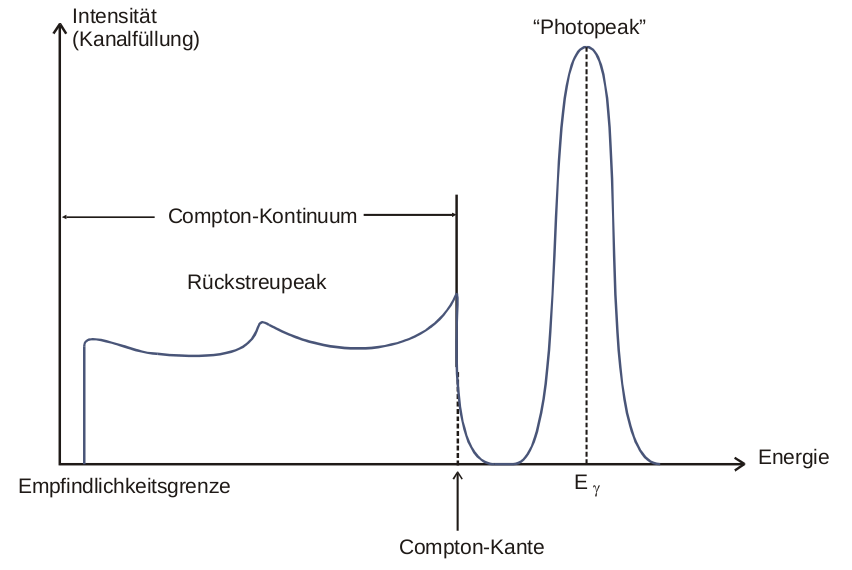
\includegraphics[scale=0.3]{content/spektrum.png}
    \caption{Spektrum eines monochromatischen Photonenstrahlers der Energie $E_\gamma$ aufgenommen mit einem Germanium Detektor [1].}
    \label{fig:spektrum}
\end{figure}

Die Komponenten dieses Spektrums sind der Photopeak, das Compton-Kontinuum mit der Compton-Kante und dem Rückstreupeak. Der Photopeak entsteht, 
wenn die gesamte Photonenenergie im Detektor deponiert wird. Dieser kann demnach nur beim Photoeffekt entstehen. Somit ist der Photopeak die 
Größe von Interesse, deren Halbwertsbreite ein Maß für die Energieauflösung des Detektors ist. Das Compton-Kontinuum ist bei der Spektroskopie
eher störend. Auch oberhalb der Compton-Kante kann aufgrund von mehrfahr gestreuten Quanten eine Intensität beobachtet werden. Die Lage der 
Compton-Kante ist durch Gleichung \eqref{eqn:Kante} gegeben. Der Rückstreupeak entsteht durch Quanten, die den Detektor nicht direkt, sondern
durch Compton-Streuung in der Detektorumgebung erreichen. Auf Grund der hohen Energieschwelle der Paarbildung, spielt diese hier kaum eine 
Rolle. 

\cite{sample}
